\chapter{Application context}\label{chap:xenocontest}

\section{Introduction}

In pathology, a tumor is an abnormal mass of tissue that grows in excess and in an uncoordinated mode with respect to normal tissues, and persists in this state after the termination of the stimuli that have led the process, making it hereditary damage, against new cells.

For a cell becomes cancerous, it must accumulate a series of damages to its system of control of reproduction. In fact, cancer is a genetic disease of somatic cells. Every cancerous cells show alterations, often very large,of their chromosome structure: the number of chromosomes in the nucleus can be altered and their chromosomes are damaged, missing or multiple. Cancer can affect all tissues, especially those subject to various stress and subject to continuous exchange, as, for example, skin, respiratory tract and intestine.

The colorectal cancer (\textit{CCR}) is widespread, with high mortality in Western countries. Is the second leading cause of death among cancer patients, both in man and woman. The incidence shows considerable variation according to different geographical areas. In the U.S. it settles on 45-50 cases per 100,000 population per year, in the UK is around 25-30 cases, while in Japan does not exceed 10-12 cases per 100,000 inhabitants per year. Italy is among the countries with intermediate incidence rate, with about 35 cases per 100,000 population per year and presents significant differences from region to region. The CCR is rare under the age of 50, and its incidence increases rapidly with age, doubling every decade between 40 and 70 years. The average age at diagnosis is about 69 years old for men and 72 years old for women.

The IRCC is an institute of Candiolo responsible for research and treatment of cancer. At the institute, are conducted several experimental protocols, with the use of laboratory experimental mice in order to identify and develop new treatments for cancer. Research studies currently are focusing on colorectal cancer (CCR).

\section{Approaches to cancer - Target Therapy}

The main problem in cancer therapy is that, in general, being a cancer composed of cell essentially very similar (if not for some genetic damage) to the rest of the body, drugs active against cancer cells are usually also very toxic to normal cells. For this reason, a fundamental objective in oncology research is by the action \textit{targeted drugs}, resulting in a therapeutic window. Any drug developed for act against cancer cells must be tested carefully to make sure also that will not damage healthy cells in the body.

The high rate of replication of cancerous cells makes them more vulnerable to radiation than normal tissue. This weakness is exploited to heal many types of solid tumor with radiation (\textit{radiotherapy}, bombardment with gamma rays) in an effort to kill as many cancer cells as possible. On other hand, the \textit{chemiotherapy} exploits the sensitivity of individual tumors to specific substances. Since the sensitivity of the tumor depends also on the patient's immune system is usually designed a custom blend of several drugs for each patient. Almost always, this cocktail contains one or more inhibitors of mitosis, such as taxol and its derivatives to prevent cellular proliferation. Some of these inhibitors are primarily responsible for alopecia (hair loss ) that afflicts patients undergoing chemiotherapy.

The cancer develops and progresses as a result of a genetic lesion, that is an alteration of the DNA in an adult cell. So turn off the genetic lesion that produced the means compromising tumor its growth. The targeted therapies, developed over the past 20 years, are indeed able to block the function of genetically altered molecules in the tumor without affecting normal tissues and therefore without causing a general body damage.

These therapies are useful only in subjects with a tumor that contains, in the DNA, the anomaly which makes the tumor susceptible to the drug targeted. This approach also has diagnostic and therapeutic challenges, necessarily, the traditional classification of neoplastic diseases.

In the context of cancer therapy targets are no longer defined by place of occurrence and morphological characteristics, but also on the basis of the molecular lesion that characterizes them and , at the same time, makes them vulnerable to a particular treatment. New therapies are therefore not only targeted, but also personalized. The molecular diagnosis refers to the need to precisely characterize each patient for various genetic mutations that presents the tumor and, therefore, makes it sensitive to a drug and resistant to others.

\section{Xenopatients}\label{sez:xp}

At the Institute of Candiolo it was decided to create a platform for preclinical investigations which best approximates the context of real tumors. The project involves the recovery of surgical pieces (samples) from surgery, with the informed consent of patients. The sample is stored under conditions that ensure the vitality and then is implanted in a receiving animal, usually under the skin of an experimental mouse. The animal becomes a "small patient" that is subjected to experimental therapies. For this, we define the mouse that brings with it the human cancer \textbf{xenopatient}. The choice fell on mice because they have a DNA structure very similar to that of humans. In addition, allow for a wide range of organisms on which to make tests at a reduced cost. Finally, these mice are delivered already immunosuppressed, with the immune system very weak, so they are more susceptible to other infections, because their weakest.

The experimental animals are farmed directly in the institution (to make economically sustainable the research), through the maintenance of a breeding colony (\textbf{breeding}) that generates the animals on which experiments are actually carried out (\textbf{experimental}).

The study enables the execution of \textbf{large-scale genetic analysis} of the tumor, in order to identify lesions that potentially are susceptible to attack with the experimental drugs. In the presence of a lesion, the xenopatient is treated with the drug target and response to treatment is monitored. In case of positive result the next step is to transfer the information to the clinic and begin to treat real patients (but only those with the genetic defect that responds to therapy) with the drug that has shown efficacy in xenopatients. In other words, the preclinical xenopatients allow the personalization of targeted therapies.

Among the available drugs for the treatment of colorectal cancer, cancer of the head and neck and, according to recent studies, also lung cancer, is administered the \textbf{Cetuximab}, a monoclonal drug, produced in a mammalian cell line by recombinant DNA techniques. Even the IRCC of Candiolo used this drug, testing it on patients and on xenopatients.

Efficacy evidence of the Cetuximab as a treatment of colorectal cancer are numerous. With the administration of this drug, alone or in combination with traditional chemotherapy drugs, in patients refractory to classical treatments (chemotherapy alone), is achieved an increase in response rate, disease control, disease-free survival.

Even when used in first line (early in the disease), has been shown to increase the positive effects of the chemotherapy also to allowing more patients to achieve a reduction in tumor size. Unfortunately, not all the population that the drug is administered benefits from the positive effects of Cetuximab. For this reason a number of years of scientific research is investigating the possible existence of factors that can predict response to therapy. Although some markers have been identified predictors, to date there is no marker that can identify with sufficient sensitivity and specificity patients who respond adequately to treatment with Cetuximab. The identification of these markers would be extremely useful to apply the medication in a selected population is under the first line and second-line allowing you to reduce costs, avoid non-responding patients to unnecessary treatment burdened by adverse effects and improve the selection of personalized therapies

The key point in order to conduct the study is to obtain a good engraftment of the tumor samples in mice. As can be imagined, if the tumor will not grow in the tissues of xenopatients, can not do experiments. The goals of these operations are basically two. The first consists in the expansion of tumor material, with the purpose of collection material. The second, however, meets the objective of having to perform experimental treatments.
In the figure~\ref{fig:schema} is shows the general pattern of the flow of operations on xenopatients, placed in the context of the institution. 
%Below are detailed steps in the image.
\begin{figure}[h]
\begin{center}
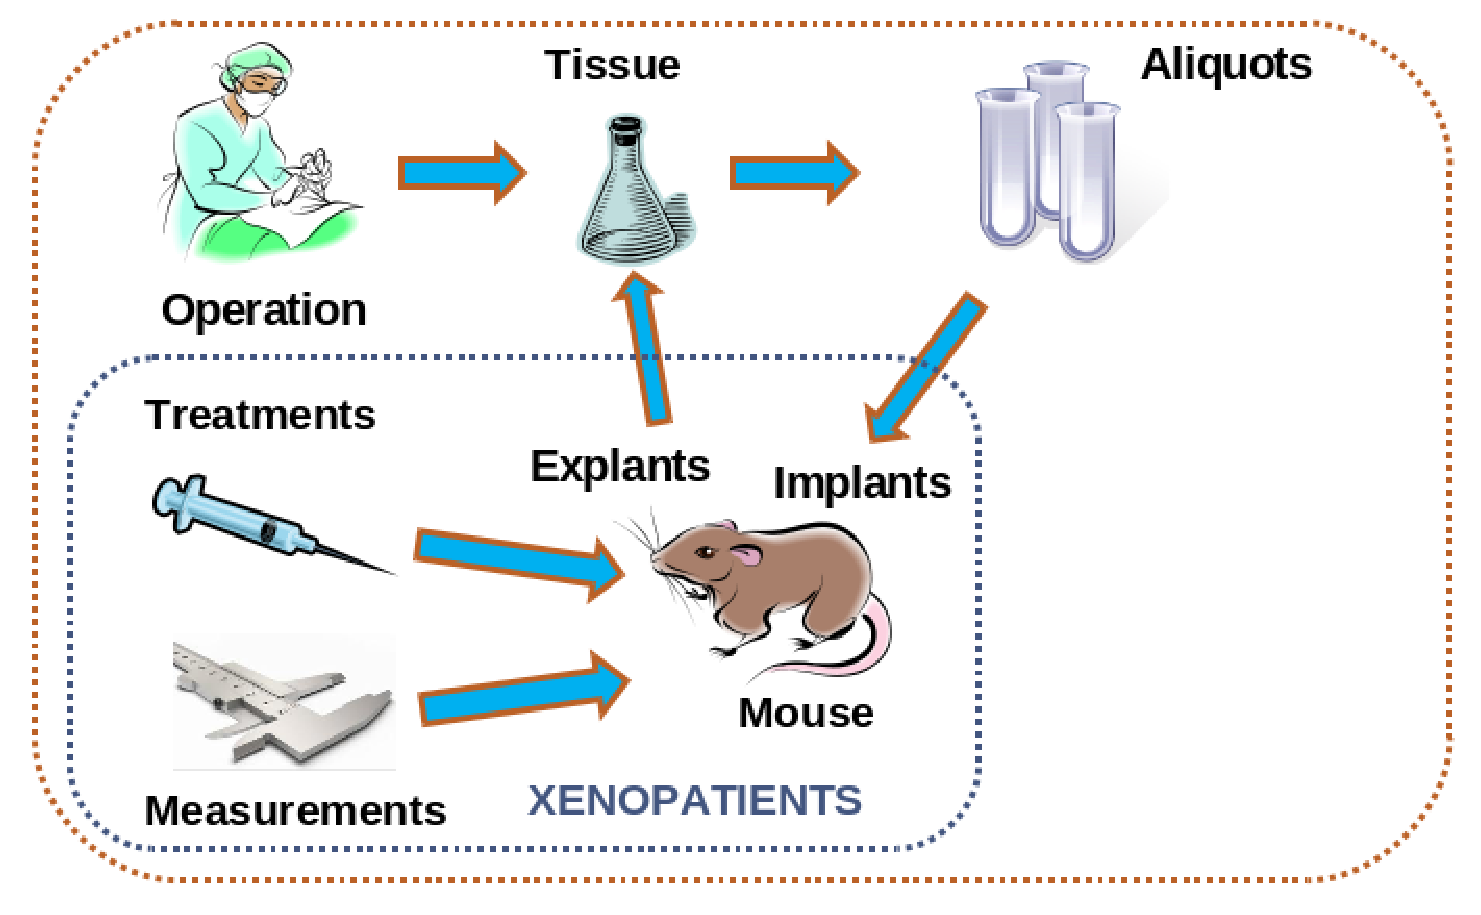
\includegraphics[width=0.8\textwidth]{./Figure/schema}
\end{center}
\caption{Operational flow on the xenopatients}\label{fig:schema}
\end{figure}

The procedure adopted involves various stages. The first takes place in the surgery room where surgery is the sample collected fresh.

Later, in conditions close to the maximum sterility, it's taken a part of the sample of tumor, and then divide the portion into several fragments. Each fragment is stored inside the tubes. Thereafter, the samples are brought to the operating table veterinarian for \textit{implant} in mice. The aims of the plants may be testing some drugs or the production of tumor tissue, using mice as an incubator.

To evaluate the efficacy of \textit{treatment} with the targeted drug, it is necessary to derive from a single tumor xenopatients a court sufficiently large to be divided into two groups, one of the treaties and that of the untreated (\textit{control group}).

A treatment is the administration of one or more drugs to xenopatients, with a precise scheduling and length of time. We also distinguish \textit{acute treatments}, which require mandatory explant of mice on which they are performed, ​​in order to identify and study the behavior of biomarkers in drug response.

Controls are carried out on tumor growth by palpation of the lesion in the plant or by measuring with a caliber. With these measurements it is possible to evaluate the effectiveness of a treatment . In fact, If there is a slowdown or a halt in tumor growth, it appears that the treatment is achieving the goal.

Then, there comes the sacrifice of the mice through a lethal dose of anesthetic. The tumor is removed and it is divided into several fragments. It performs this procedure for each of the implanted xenopatients for which explant is requiredo.

Through the operation from explant of the tumor by xenopatients, is possible create a variety of new rates to be, for example, implanted in other mice. Doing so creates an evolution of the original tumor, passing from mouse to mouse, and keeping it alive. On this basis, we can introduce the concept of genealogy of xenopatients. They belong to the same lineage the mice that received the same plant tissue, derived from a single progenitor xenopatients. Taking advantage of the genealogy of the tumor, it is possible see its progress in the different generations, with different responses to various treatments and engraftment.

\ Xeno \ born in this context, with the aim of managing the data on of xenopatients and, in particular, all the information about the life cycle of a mouse, such as measurements and pharmacological treatments. Although current studies are focused on the CCR, the developed application is able to manage all information relating to of xenopatients regardless of the type of cancer studied.